\section{Computational Methods}

This section focuses on practical computational approaches to implementing the James-Stein Estimator and Ridge Regression. Through simulations and comparisons, we demonstrate the effectiveness of these methods in statistical estimation.

\subsection{Implementing James-Stein Estimator}

The James-Stein Estimator is implemented to demonstrate its shrinkage effect on simulated data. This estimator is particularly notable for its ability to reduce estimation errors by shrinking estimates towards their overall mean.

\subsubsection{Algorithm for James-Stein Estimator}
\begin{algorithm}
\caption{James-Stein Estimator}
\begin{algorithmic}[1]
\Procedure{JamesSteinEstimator}{$z$, $sigma\_squared$}
    \State $n \gets \text{length}(z)$
    \State $z\_bar \gets \text{mean}(z)$
    \State $s\_squared \gets \text{sum}((z - z\_bar)^2) / n$
    \State $shrinkage\_factor \gets 1 - ((n-3) * sigma\_squared / s\_squared)$
    \State $shrinkage\_factor \gets \text{max}(0, shrinkage\_factor)$
    \For{$i \gets 1$ to $n$}
        \State $z[i] \gets z\_bar + shrinkage\_factor * (z[i] - z\_bar)$
    \EndFor
    \State \textbf{return} $z$
\EndProcedure
\end{algorithmic}
\end{algorithm}

\subsubsection{Simulation Results}

Data are generated from a normal distribution with a mean of 5 and a standard deviation of 1. The James-Stein Estimator is then applied to these data, demonstrating significant shrinkage of estimates towards the mean. The impact of this shrinkage is clearly illustrated in a scatter plot that compares the original data with the James-Stein estimation.

\begin{figure}[H]
    \centering
    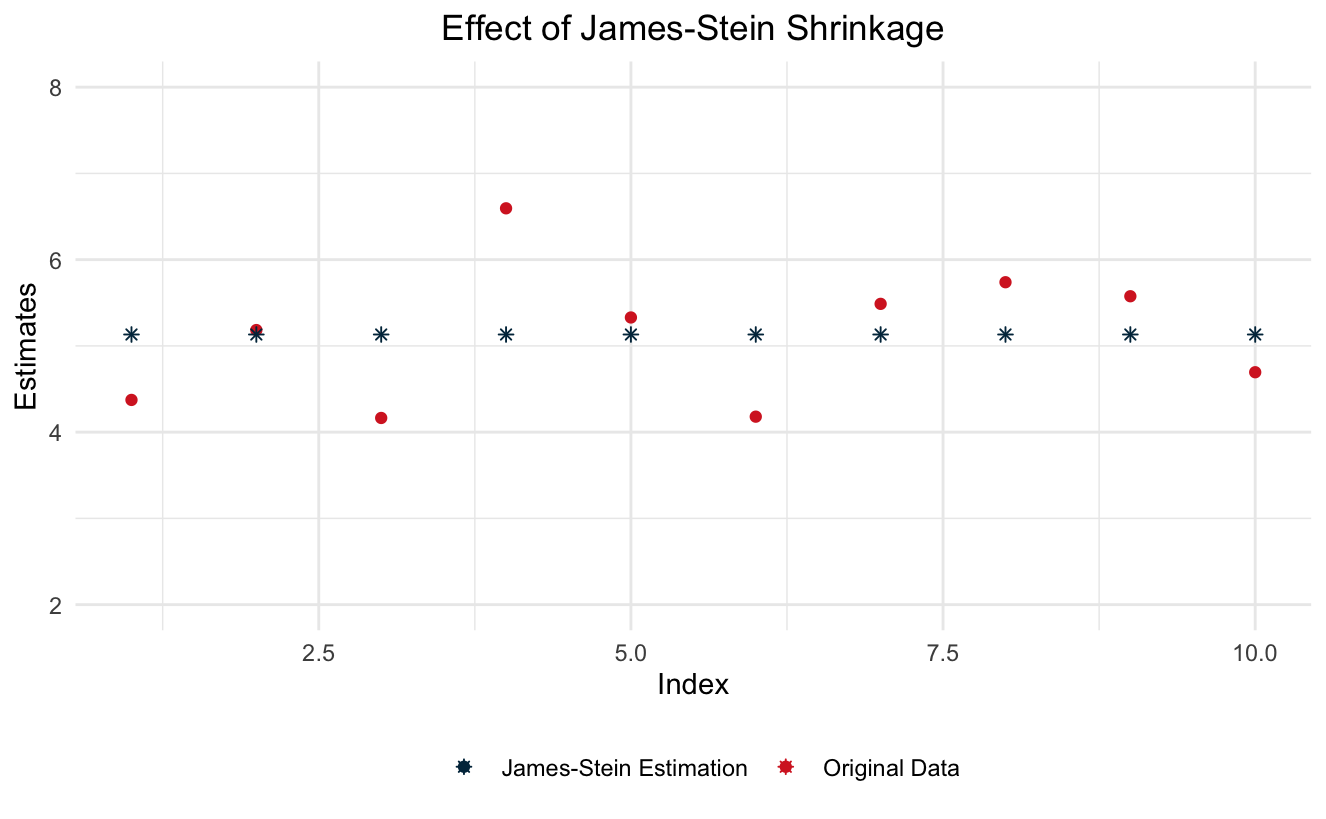
\includegraphics[width=1\textwidth]{Effect of James-Stein Shrinkage.png}
    \caption{Effect of James-Stein shrinkage on simulated data.}
    \label{fig:jse_shrinkage}
\end{figure}

\subsection{Simulation of Estimator Effectiveness}

We compare the James-Stein Estimator with the Maximum Likelihood Estimator across different sample sizes to illustrate the reduction in squared errors.

\newpage

\subsubsection{Algorithm for Comparing Estimator Effectiveness}
\begin{algorithm}
\caption{Compare Estimators}
\begin{algorithmic}[1]
\Procedure{CompareEstimators}{$num\_sim$, $sample\_sizes$, $mu$, $sigma$}
    \For{$n$ in $sample\_sizes$}
        \State $mle\_errors \gets$ vector of size $num\_sim$
        \State $jse\_errors \gets$ vector of size $num\_sim$
        \For{$i \gets 1$ to $num\_sim$}
            \State $z \gets \text{generate normal data}(n, mu, sigma)$
            \State $mle \gets \text{mean}(z)$
            \State $s\_squared \gets \text{sum}((z - mle)^2) / n$
            \State $shrinkage\_factor \gets 1 - ((n-3) * sigma^2 / s\_squared)$
            \State $shrinkage\_factor \gets \text{max}(0, shrinkage\_factor)$
            \State $jse \gets mle + shrinkage\_factor * (z - mle)$
            \State $mle\_errors[i] \gets \text{sum}((mle - mu)^2)$
            \State $jse\_errors[i] \gets \text{sum}((jse - mu)^2)$
        \EndFor
        \State Store $mle\_errors$ and $jse\_errors$ in data frame
    \EndFor
    \State \textbf{return} data frame
\EndProcedure
\end{algorithmic}
\end{algorithm}

\subsubsection{Visualizing Comparison Results}

The log-squared errors of both estimators are plotted to show the James-Stein Estimator's efficiency, especially in smaller samples.

Generally, the James-Stein Estimator demonstrates lower median log squared errors compared to the MLE across all sample sizes, particularly as the sample size increases. This demonstrates the effectiveness of the James-Stein shrinkage, especially in reducing variance and improving estimation accuracy over the traditional MLE approach.

\begin{figure}[H]
    \centering
    \includegraphics[width=1\textwidth]{Comparison of MLE and James–Stein Estimator Errors.png}
    \caption{Log-squared error comparison of MLE and JSE across different sample sizes.}
    \label{fig:estimators_comparison}
\end{figure}

\subsection{Exploring Ridge Regression}

Ridge Regression is investigated as an auxiliary method that also demonstrates shrinkage, similar to the James-Stein approach, but within the framework of regression analysis. Data and coefficients are generated and Ridge Regression is implemented using the glmnet package in R.

The plot of coefficient shrinkage, as the regularization parameter increases, showcases Ridge Regression's capacity to effectively manage overfitting and multicollinearity, highlighting its utility in high-dimensional statistical modeling.

\begin{figure}[H]
    \centering
    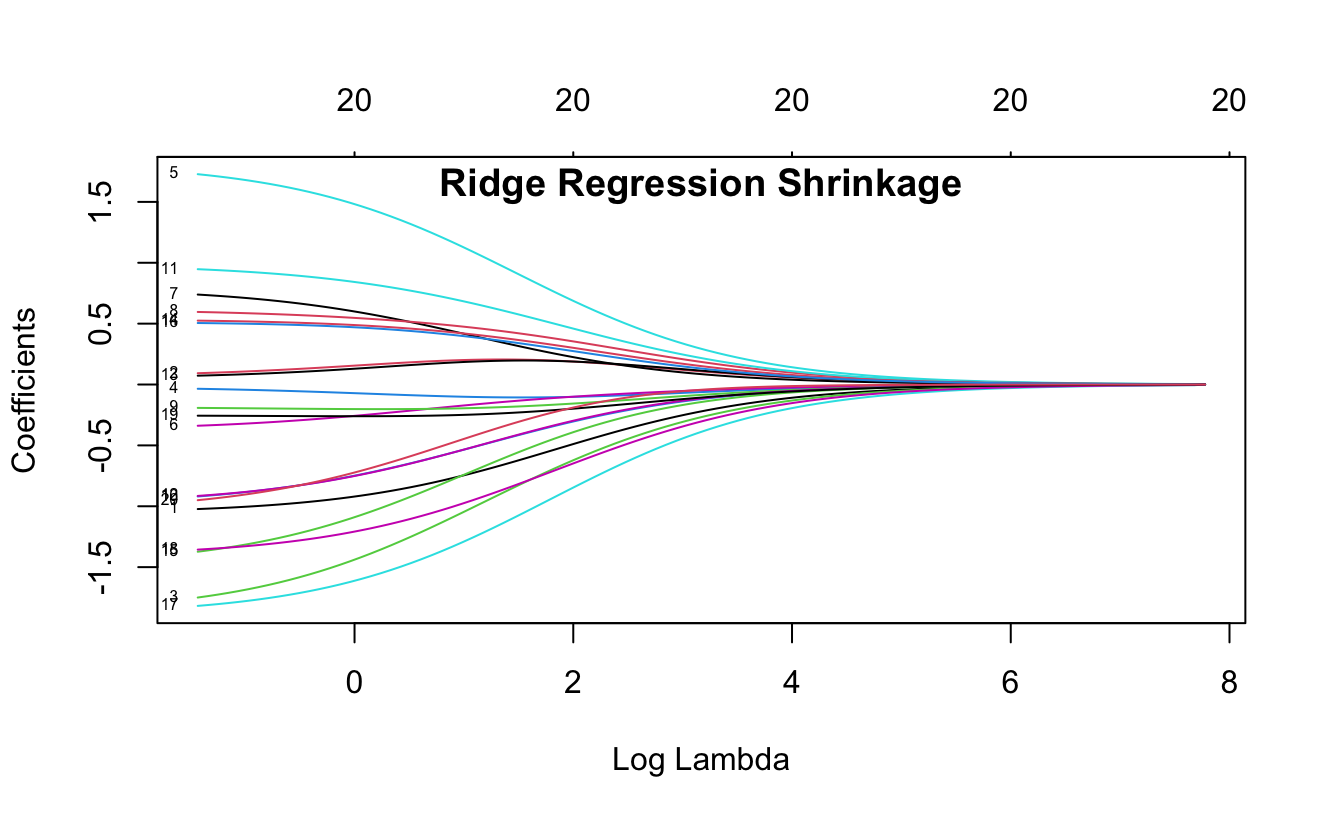
\includegraphics[width=1\textwidth]{Ridge Regression Shrinkage.png}
    \caption{Coefficient shrinkage in Ridge Regression as a function of the regularization parameter.}
    \label{fig:ridge_shrinkage}
\end{figure}

\subsection{Conclusion}

This section has showcased the practical utility and advantages of the James-Stein Estimator and Ridge Regression through detailed computational demonstrations. Both methods are united by their use of shrinkage to enhance the accuracy and dependability of statistical estimates.